% Autor: João Fiuza de Alencastro
% Disciplina: Segurança de Redes
% Relatório 3
\documentclass[journal]{IEEEtran}
\usepackage{listings}
\usepackage[utf8]{inputenc}
\usepackage{graphicx}
\usepackage[colorlinks=true,urlcolor=red,citecolor=blue,linkcolor=blue]{hyperref}




\begin{document}

\title{Relatório OWASP}


\author{João~Fiuza~de~Alencastro~15/0131933}% <-this % stops a space




% make the title area
\maketitle


\begin{abstract}
Relatório destinado à matéria de Segurança de Redes do Departamento de engenharia Elétrica da Universidade de Brasília. Experimento realizado a fim de explorar vulnerabilidades expostas pela OWASP em uma aplicação específica para testes.
\end{abstract}

\begin{IEEEkeywords}
Segurança, redes, OWASP, ZAP, XSS, Wordpress, injection, top ten, juice shop.
\end{IEEEkeywords}


\IEEEpeerreviewmaketitle



\section{Introduction}
\IEEEPARstart{U}{tilzar} das vulnerabilidades mais exploradas na atualidade em uma aplicação privada que simula ambientes reais. \par
No mundo da computação, diferentes tecnologias vão e vêm, sempre junto à elas, acompanham suas respectivas vulnerabilidades. Logo, assim que são descobertas grandes falhas de segurança generalizadas, ou elas podem ser exploradas por pessoas com essas informações privilegiadas, ou elas são expostas pela comunidade para que todos possam se tomar as devidas medidas de segurança. \par
A OWASP (Open Web Application Security Project) é uma organização, sem fins lucrativos, mundialmente reconhecida focada em melhorar a segurança de software. Seu propósito é ajudar indivíduos, entidades e organizações a se protegerem contra os males infiltrados no mundo da computação.\par
Todos os anos a OWASP libera uma nota oficial listando as principais vulnerabilidades que estão sendo exploradas. Esta lista representa uma das 'Top Ten' ameaças lançadas pelo OWASP e reconhecidas por grandes organizações. O propósito dessa lista não é ajudar ou dar ideias aos atacantes e à pessoas mal-intencionadas, mas sim aos mantenedores de softwares que desejam se proteger de ameaças novas, porém já vastamente exploradas. \par
Neste experimentos utilizaremos a lista abaixo como ponto de partida para explorarmos cada item, descobrindo se há a vulnerabilidade ou não. As principais ferramentas que serão utilizadas serão o WPScan e o OWASP ZAP. \\

\begin{itemize}
\item[--] A1 Injection 
\item[--] A2 Broken Authentication and Session Management 
\item[--] A3 Cross-Site Scripting (XSS) 
\item[--] A4 Insecure Direct Object References 
\item[--] A5 Security Misconfiguration 
\item[--] A6 Sensitive Data Exposure 
\item[--] A7 Missing Function Level Access Control 
\item[--] A8 Cross-Site Request Forgery (CSRF) 
\item[--] A9 Using Components with Known Vulnerabilities 
\item[--] A10 Unvalidated Redirects and Forwards \ldots
\end{itemize}


\subsection{Montando o ambiente}
\subsubsection{Juice shop}
O Juice shop é uma aplicação escrita em Node.js, Express e Angular listada no diretório VWA OWASP. Foi criada para treinamentos na área de segurança, intecionalmente vulnerável e com várias falhas a serem exploradas. Algumas dessas falhas são as listadas no top ten da OWASP. Uma de suas vantagens é que representa extremamente bem ambientes em produção muito utilizados atualmente. Esse é o ambiente de testes que será utilizado neste experimento.
\\
\subsubsection{Docker}
O Docker é uma ferramenta de "containerização", ela realiza um tipo de virtualização a nível de sistema operacional mantendo uma comunicação a nível de aplicação com o kernel do sistema hospedeiro. O Docker será utilizado para criar um container da aplicação do juice shop, desta forma, será possível fazer todos os testes necessários na própria máquina local. \par
A imagem utilizada foi retirada do repositório público oficial do criador da aplicação no DockerHub [3]. Uma vez feito o download, basta somente um comando no terminal para deixar tudo pronto: \\
\begin{lstlisting}[language=bash]
$ docker run --rm -p 3000:3000 \
> bkimminich/juice-shop
\end{lstlisting}

\subsubsection{Wordpress}
No experimento realizado em sala de aula, foi fornecido aos alunos um ambiente muito comum para websites ou blogs, um Wordpress. Como é uma aplicação web extremamente difundida nos dias de hoje, é normal que haja diversas vulnerabilidades expostas, tantas que há um software de scan específico para o Wordpress, o wpscan, já instalado por padrão no kali linux. 

\subsection{Procurando vulnerabilidades}
\subsubsection{OWASP ZAP}
Zed Attack Proxy (ZAP) é uma ferramenta de segurança mantida por inúmeros voluntários. Ela pode ser de grande ajuda quando se trata de encontrar vulnerabilidades em aplicações web a fins de desenvolvimento e testes, também é de grande uso para hackers éticos e testes de penetração. \par
Este foi o primeiro passo na realização dos testes do experimento, foi feita uma varredura com essa ferramenta em nosso juice-shop. Na figura 1, pode-se verificar que foi encontrada uma informação valiosa dentro de um dos arquivos java-script. Algo que em mãos erradas pode causar danos irreparáveis. Foi exposto um endereço IP interno da aplicação, além disso, o protocolo utilizado é um http sem segurança alguma. Uma vez que um indivíduo mal intencionado tem posse dessa informação, ele poderá enviar pacotes infectados para dentro da rede da aplicação com um alvo já preparado.
\par
Além de descobertas de IP, a ferramenta pode achar muitas outras coisas. Ainda na mesma figura 1, pode-se verificar na aba de alertas, descobertas como, autocomplete de senhas no browser, proteção contra XSS desabilitada, dentre outros.

%Imagem
\begin{figure}[h!]
	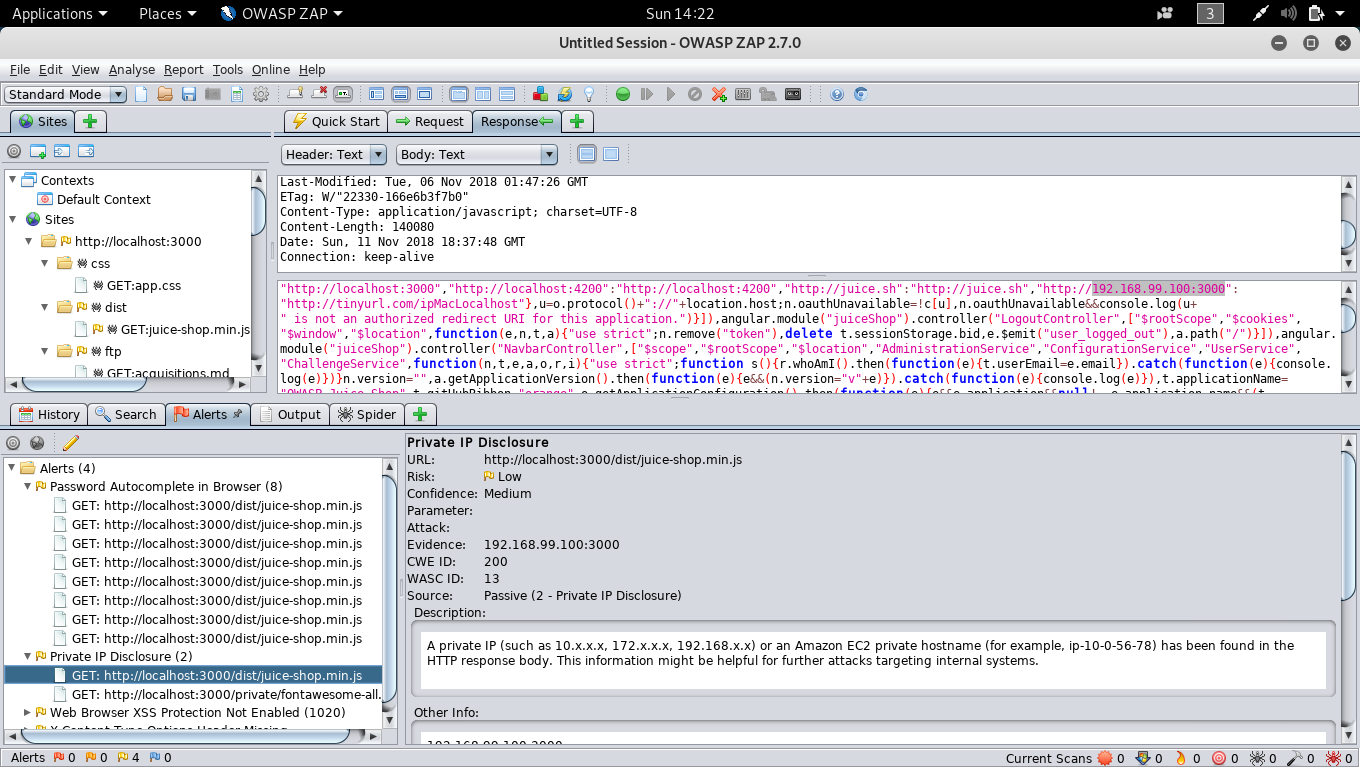
\includegraphics[width=\linewidth]{../fotos/juice_shop/private_IP_found.png}
	\caption{IP privado exposto}
	\label{fig:private_ip}
\end{figure}

Uma prova de que a varredura foi bem sucedida é fornecida pelo lado da vítima, nesse caso o Juice-shop dá um 'feedback' para o treinamento à medida que ele é bem sucedido. Na figura 2 é verificado que a varredura do ZAP realmente acessou arquivos e códigos que não foram feitos para serem públicos.

%Imagem
\begin{figure}[h!]
	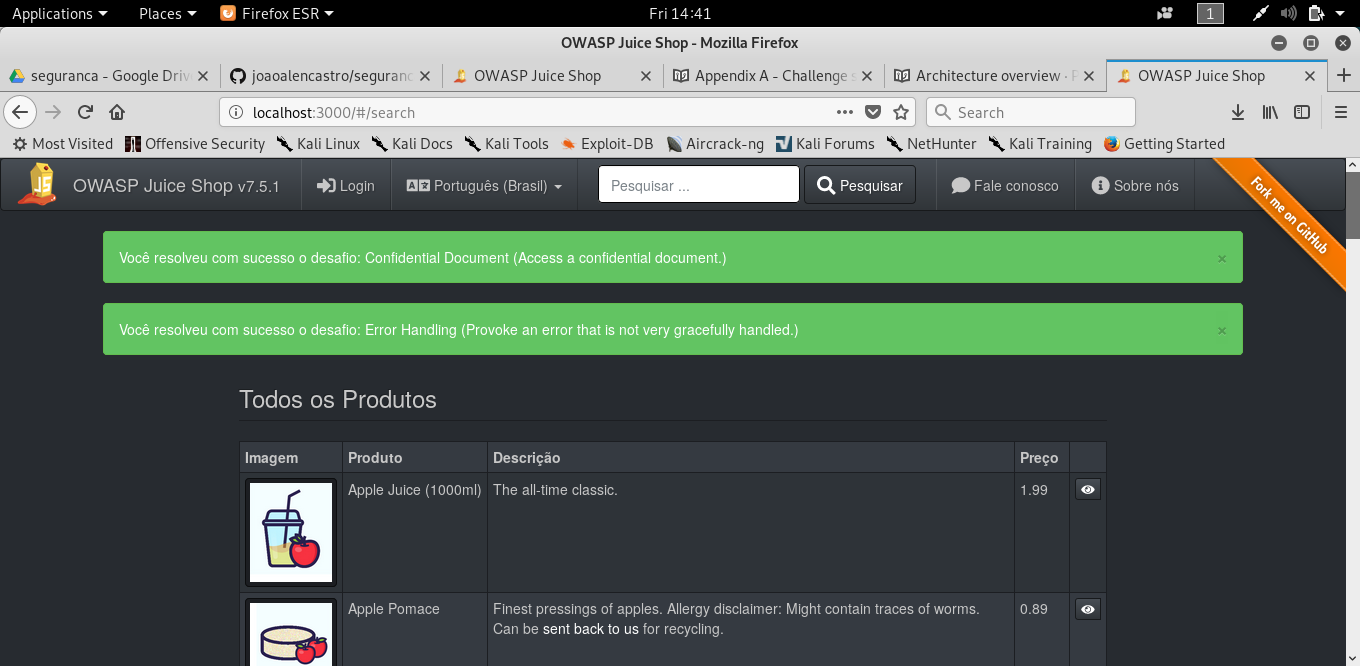
\includegraphics[width=\linewidth]{../fotos/juice_shop/desafio_juice_shop.png}
	\caption{Desafio juice shop bem sucedido}
	\label{fig:successful_challenge}
\end{figure}

Em sala de aula foram obtidos vários resultados de uma varredura no Wordpress, também foi utilizado o OWASP ZAP em uma primeira análise mais superficial. É possível notar resultados interessantes, porém são descobertas superficiais, é necessário ter resultados mais específicos. A figra abaixo mostra os alertas apontados pela ferramenta.

%Imagem
\begin{figure}[h!]
	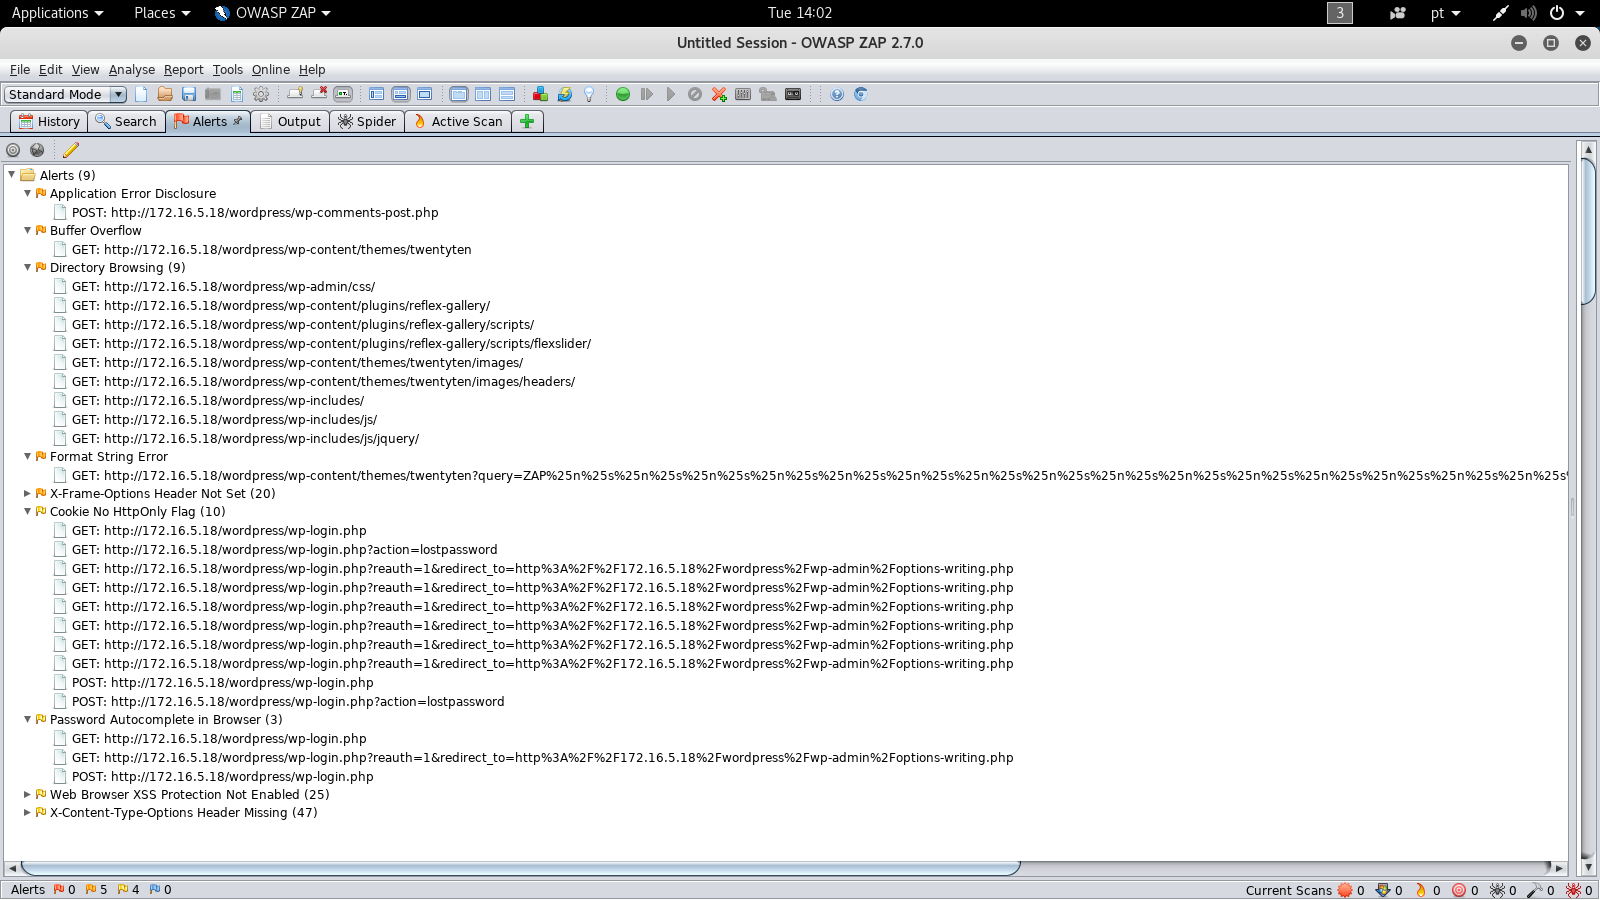
\includegraphics[width=\linewidth]{../fotos/OWASP_ZAP_FOTOS/zap_alerts.png}
	\caption{Alertas apontados no wordpress}
	\label{fig:wordpress_alerts}
\end{figure}

\subsection{Explorando o Wordpress}
Ao utilizar ferramentas mais específicas, as possibilidades de ataque contra o wordpress aumentam significativamente. Descobre-se a versão do wordpress, todos os algorítmos de interação utilizados, com essas informações é possível rodar diferentes programas de ataque contra essa aplicação. Na imagem abaixo é listado ataques como: SQL injection, Transversal Directory DoS, Long Password DoS, REST API Content Injection, e muitos outros.

%Imagem
\begin{figure}[h!]
	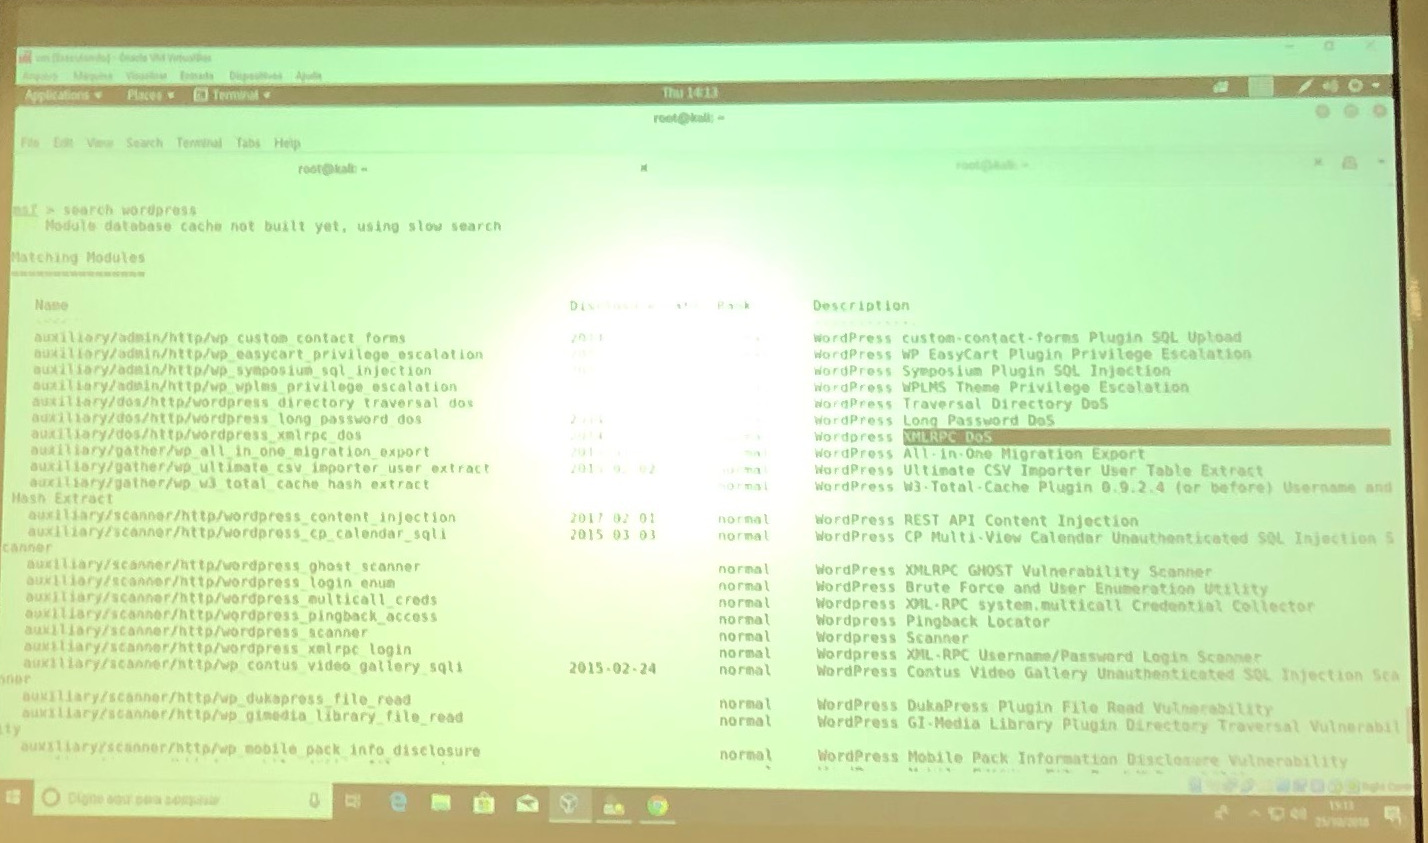
\includegraphics[width=\linewidth]{../fotos/wpscan/IMG_8233.JPG}
	\caption{Vulnerabilidades do wordpress}
	\label{fig:wordpress_vulnerabilities}
\end{figure}

A partir dessas informações foi possível realizar ataques à aplicação do wordpress. Uma delas foi um simples DoS, impossibilitando o servidor de responder a outras requisições, consequentemente o tirando do ar. Mostrando que essa simples aplicação web não tem defesas do tipo de negação de serviço, um grande erro. Outro ataque realizado foi um SSH reverso aplicado na máquina em questão, dessa maneira, é possível burlar o sistema do Firewall, o qual recusa qualquer requisição de fora desconhecida na porta 22. Escolha extremamente falha, já que o firewall não bloqueia conexões de dentro para fora. A solução para esse problema seria criar um regra bi-direcional no firewall, solução simples e efetiva.

\subsection{Cross-Site Scripting (XSS)}
Uma das tenebrosas vulnerabilidades na atualidade é a Cross-Site Scripting, conhecido com XSS. Esse tipo de ataque se resume em scripts maliciosos inseridos no ambiente que rodam no lado do cliente. Um pequeno código java-script pode fazer grandes estragos e expor informações pessoais de usuários finais.\par
Foi realizado um simples ataque XSS no juice-shop da forma banal. Pelo fato de não haver um filtro de strings na inserção de textos do front-end, é possível executar pedaços de código no navegador do usuário, como mostrado nas figura 5 e 6.

%Imagem
\begin{figure}[h!]
	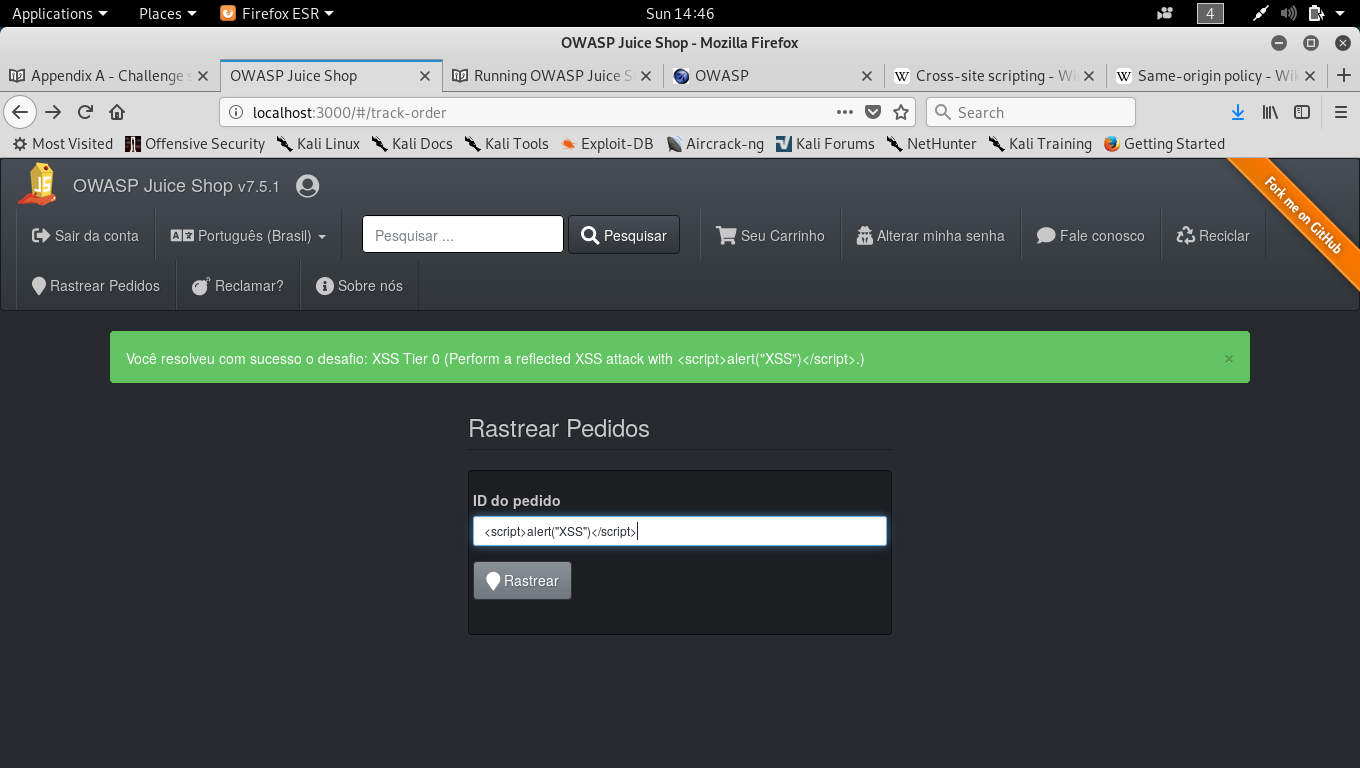
\includegraphics[width=\linewidth]{../fotos/juice_shop/simple_XSS_1.png}
	\caption{Simples XSS}
	\label{fig:simple_xss_1}
\end{figure}

%Imagem
\begin{figure}[h!]
	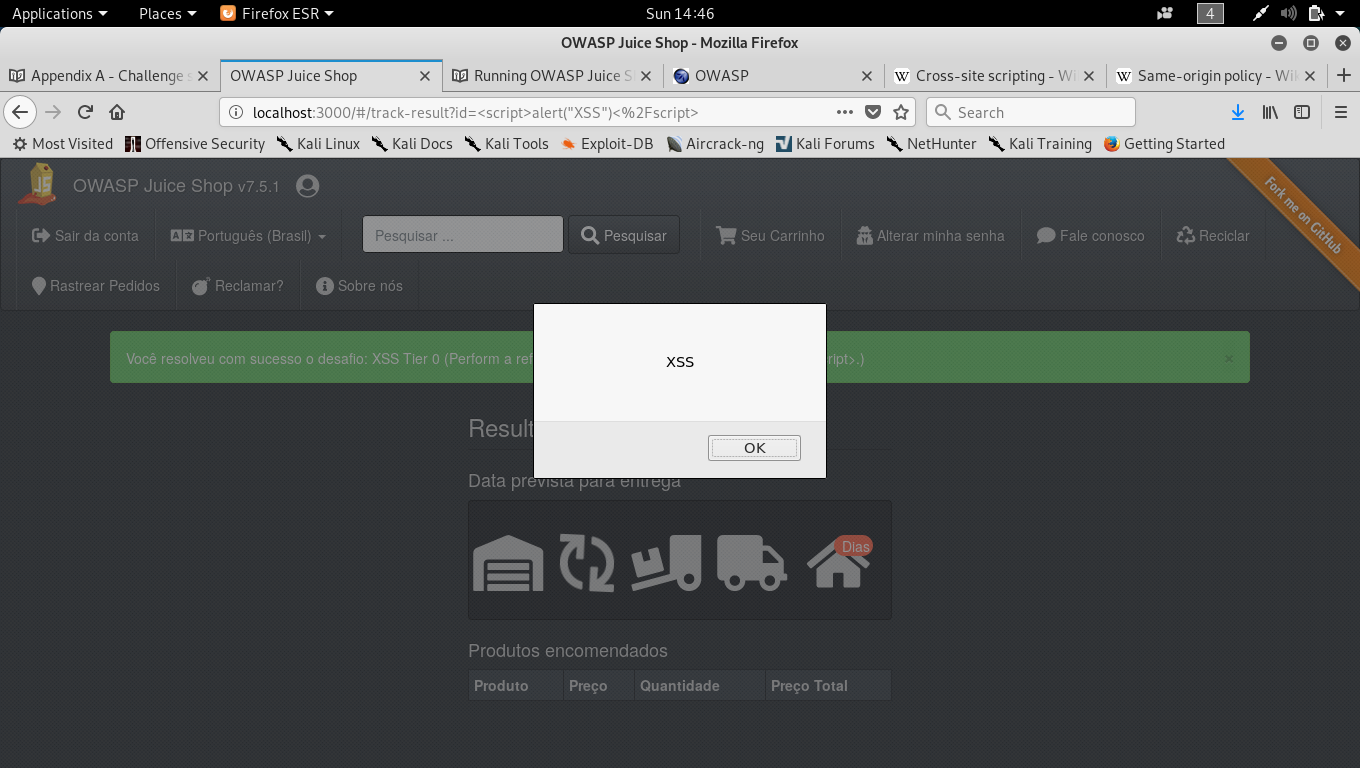
\includegraphics[width=\linewidth]{../fotos/juice_shop/simple_XSS_2.png}
	\caption{Resultado: Simples XSS}
	\label{fig:simple_xss_2}
\end{figure}

Pode parecer um ataque inofensível, afinal o que pode um alerta fazer? Porém, é extremamente perigoso, o ponto importante é que foi executado um código malicioso no navegador do usuário, independentemente de ser um simples alerta. O XSS pode ser usado para 'driblar' controles de acesso, como a política da mesma origem.

\subsection{Acessando informações de outro usuário}
Utilizando apenas as ferramentas presentes no navegador é possível alterar informações da aplicação, mudando flags de sessão. No exemplo apresentado abaixo, é mudado um pequeno valor de chave chamada "bid" no armazenamento de sessão.

%Imagem
\begin{figure}[h!]
	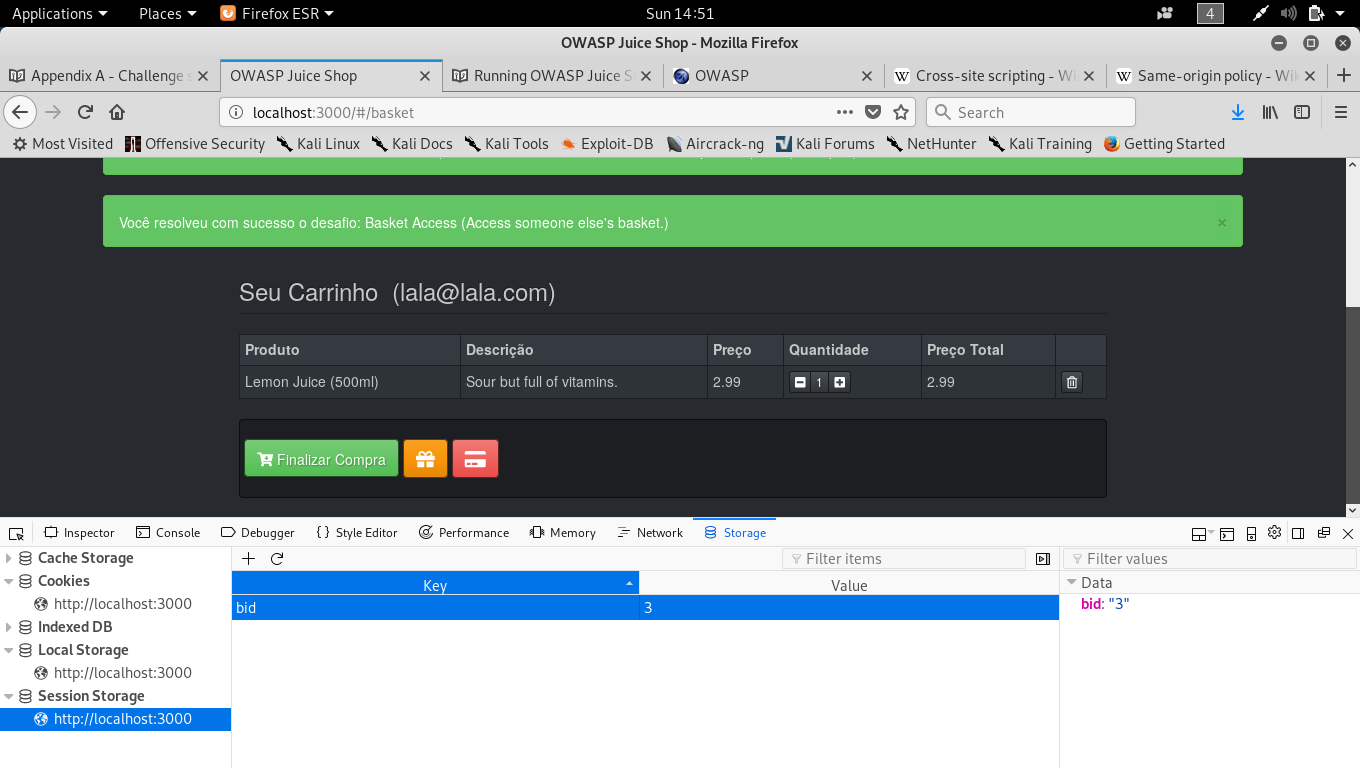
\includegraphics[width=\linewidth]{../fotos/juice_shop/storage_value_changed.png}
	\caption{Valor de armazenamento alterado}
	\label{fig:storage_value_changed}
\end{figure}

%Imagem
\begin{figure}[h!]
	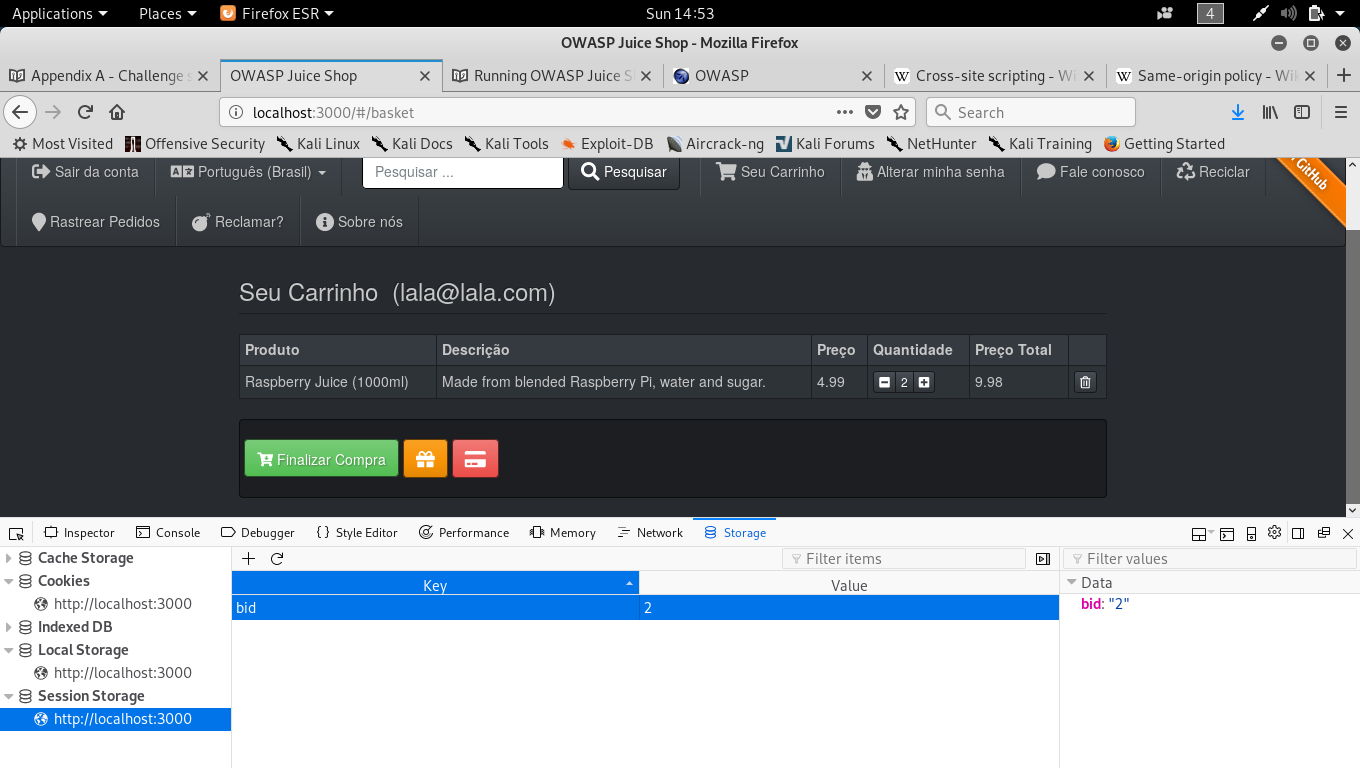
\includegraphics[width=\linewidth]{../fotos/juice_shop/storage_value_changed_2.png}
	\caption{Resultado: Valor de armazenamento alterado}
	\label{fig:storage_value_changed_2}
\end{figure}

Uma simples flag de inteiro pode alterar todo um carrinho de compras, fazer com que alguém acesse as informações de outro usuário.

\section{Conclusion}
Utilizando essas e outras ferramentas, vai ficando claro como um atacante procede na atuação de um \textit{exploit}. Pode parecer que não, mas ao colocar uma aplicação web para executar publicamente, muitas informações são expostas, portanto é de extrema importância que a aplicação esteja de acordo com as proteções necessárias e disponíveis. A OWASP sempre disponibiliza informações sobre segurança, porém não há magia, segurança computacional requer esforço e dedicação, o primeiro passo para ter um sistema seguro é atualizar as aplicações assim que disponíveis.



\begin{thebibliography}{1}

\bibitem{owasp}
https://www.owasp.org
\bibitem{docker}
https://en.wikipedia.org/wiki/Docker-(software)
\bibitem{docker-hub}
https://hub.docker.com/r/bkimminich/juice-shop/
\bibitem{xss}
https://en.wikipedia.org/wiki/Cross-site-scripting


\end{thebibliography}



\end{document}


